% generated by build-tex.mjs -- do not edit by hand (source: draft-extended.full.md)
\documentclass[11pt]{article}
\usepackage[margin=1in]{geometry}
\setcounter{secnumdepth}{-\maxdimen}  % headings carry hand-written numbers; without this LaTeX prints both (reviewer A1)
\usepackage{amsmath,amssymb}
\usepackage{graphicx}
\usepackage{calc}  % pandoc emits \real{} for table column widths; calc defines it
\usepackage{booktabs,longtable,array}
\usepackage{etoolbox}
\usepackage{microtype}
\usepackage{parskip}
\usepackage[hidelinks]{hyperref}
\newcounter{none}  % pandoc emits \def\LTcaptype{none}; without this counter LaTeX errors
\providecommand{\tightlist}{\setlength{\itemsep}{0pt}\setlength{\parskip}{0pt}}  % pandoc emits \tightlist; the bare article class does not define it
\setlength{\emergencystretch}{2em}  % let lines stretch instead of overflowing
\AtBeginEnvironment{longtable}{\small\setlength{\tabcolsep}{4pt}}  % six wide tables

\title{Outcome Gates Are Direction Filters\\[4pt]
\large Under mechanical edit semantics: what result-based validation can and cannot catch — an exhaustive audit over five constructed corpora, with an edit-semantics sweep}
\author{Anan Long\\\small Independent researcher}
\date{2026-09-24}

\begin{document}
\maketitle

\begin{abstract}
A system that rewrites its own rules must decide whether each rewrite helped. In practice it re-runs and keeps whatever looks better. This paper asks what that test can actually see.

It can see the direction of the day's move, and never the reason for it. Under mechanically defined edit semantics, a result-based gate accepts a proposal exactly when the proposal moves exposure the same way the day moved (Lemma 1, one line) --- attribution does not enter the expression. The gate is a direction filter, not an attribution signal.

Because the proposal space is finite (days \ensuremath{\times} rules per semantics), we count its behaviour over all of it instead of sampling; a confidence interval here would be a category error, not a modelling choice. Across four corpora, a same-day gate admits 61/125 = 48.8\% of edits that name the wrong rule, and the rate tracks the day's type rather than the rule at fault --- 78.1\% on losing days against 18.0\% on small-win days.

The gate then fails in two opposite ways. Where the edit vocabulary can express a repair, it over-admits wrong attributions (48.8\%); where it cannot (undo-only, halve, no-leverage), it rejects up to 10 of 19 correct edits. Where a cap or clip pins the position, no single-rule edit moves it and the gate admits nothing at all --- on real days 46.4--51.1\% of proposals are such no-ops, and one window holds 158 days that reject every proposal.

On real market days (four datasets, 74,484 cells) the closed form holds with zero violations, losing days admitting 33.0--37.8\% against 13.3--16.1\%. A third party's strategy is admitted at 46.2--57.4\%, inside 50-seed permutation bands. The direction replicates; the rate is a property of the proposal mix. We evaluate no deployed gate and make no frequency claim.
\end{abstract}

\section{1. Introduction}\label{introduction}

When a trading system rewrites its own rules, something has to decide whether the rewrite was an improvement --- usually by re-running the book and keeping whatever looks better. This paper asks what that test can actually see. We isolate its narrowest judgement: given one day's loss, \emph{which rule should be changed?} Real markets provide no ground truth for that question, so we use corpora in which the ground truth is constructible and \textbf{frozen before the experiment runs}: each day carries one intended answer plus one planted bait, the answer key is hashed, and the scorer prints that hash with every reading.

Four corpora are used throughout. \textbf{A} (5 days \ensuremath{\times} 6 rules), \textbf{B} (8 days \ensuremath{\times} 8 rules, with a deliberately different mix of day types), \textbf{C} (10 days \ensuremath{\times} 8 rules, built so that every criterion is readable --- half its days state a contradiction on the same page), and \textbf{D} (4 days \ensuremath{\times} 6 rules, built so that one day's position is \emph{pinned at a cap} --- the regime §5.5 isolates). A fifth corpus, \textbf{E} (3 days \ensuremath{\times} 8 rules), is used only in §5.5: its days are deliberately pinned or control, so it stays out of the census of §4--§5 and serves as the stress test for the counting rule.

\textbf{Relation to prior work.} The closest antecedent states in passing that a validation gate ``cannot fully catch'' the overwrites that free rewriting produces (SHARP {[}3, §4.4{]}), and its ablation compares attribution-conditioned with attribution-free behaviour (an arm reporting +7.1\% and +0.73 Sharpe that collapses toward a static baseline when attribution is removed) --- but it never measures whether the attribution itself is right, and the companion line of work carries no attribution at all. Our contribution is complementary and threefold: we make that caveat \textbf{quantitative and exhaustive} (every proposal in a finite space, counted rather than sampled); we show it is \textbf{necessary rather than incidental} (Lemma 1, §3); and we exhibit the \textbf{two opposite ways it fails} (§5) together with the precondition that turns one into the other (§5.5).

\subsection{1.1 Contributions}\label{contributions}

\begin{enumerate}
\def\labelenumi{\arabic{enumi}.}
\tightlist
\item
  \textbf{A closed form for what an outcome gate can see.} Under mechanical edit semantics a result-based gate accepts a proposal exactly when the parameter change and the day's move share a sign (Lemma 1, §3). The gate is therefore a \emph{direction filter}: it reads whether the day moved with the trade, never why the trade was taken. The equivalence is verified on real data --- four datasets, 74,484 cells, zero violations (§11; §11 also records that the four are not independent samples).
\item
  \textbf{A countable instrument.} Because the set of proposals is finite (days \ensuremath{\times} rules per semantics), the gate's behaviour over it is \emph{counted}, not estimated; sampling error --- and with it the p-value framing criticised in §2 --- does not arise.
\item
  \textbf{Two opposite failure modes, and the precondition that chooses between them.} Under an inexpressive semantics the gate rejects \emph{correct} edits --- the no-leverage semantics \textbf{keeps only 9 of 19} (§5, where the pre-registered ``no correct edit is rejected'' is narrowed rather than the criterion moved) --- while accepting an edit that rewrites the book; a four-semantics sweep separates the two regimes (§5), and §5.5 isolates the precondition --- a pinned position makes the edit a no-op, so the gate admits nothing at all.
\item
  \textbf{What tightening changes.} A cross-day gate that tightens its tolerance intercepts a different set of rules and lets a different set survive; we tabulate that trade-off (§6) instead of quoting a rate, because the shift is in \emph{which} rules are caught, not in how well correct and incorrect proposals are separated.
\item
  \textbf{A replication with its boundary drawn.} The direction replicates on real days and on proposals we did not write --- a moving-average strategy ported from a public backtesting library, \textbf{25--47 proposals} per dataset (a wider parameter pair; at its default parameters the same strategy proposes only 6--10, §11.1), 46.2--57.4\% approved, with 50-seed permutation bands containing every observed figure (§11.1). The \emph{rate} is a property of the proposal mix, and no deployed pipeline's mix is available to us (§9, §11).
\end{enumerate}

\subsection{1.2 Related work}\label{related-work}

\textbf{Evaluation protocols for self-improving loops.} Wang et al.~{[}1{]} show that harness evolution is usually searched \emph{and} evaluated on the same benchmark, and that its gains shrink against budget-matched baselines and held-out tasks; S3Gym {[}2{]} likewise separates permissive exploration from strict held-out evaluation. Our work is complementary in kind: rather than asking whether a search procedure generalises, we ask what a single validation signal can see at all, and we answer by enumeration rather than by sampling.

\textbf{Outcome gates in practice.} Recent financial agents close the loop on realised portfolio feedback: SHARP {[}3{]} commits atomic rule edits and regularises them with strict walk-forward validation; EvolveTrade {[}4{]} revises a text-parameterised policy from accumulated traces and realised feedback; EVOQUANT {[}5{]} selects candidate edits through a multi-stage verification pipeline. These gates --- not any particular implementation of them --- are our object of study.

\textbf{When the criterion is the bottleneck.} Software engineering has long known that weak test suites let repair tools produce plausible but incorrect patches {[}6{]}. Backtest overfitting is the finance-side counterpart, attacked by hypothesis testing on overfitting {[}7{]}, covariance penalties {[}8{]}, data-snooping reality checks {[}9{]}, deflated performance statistics {[}10{]}, and multiple-testing corrections in the cross-section {[}11, 12{]}. We differ in kind: where these lines estimate \emph{how often} a criterion misleads, we characterise \emph{what it can detect at all} --- a closed form over the proposal space, verified on 74,484 real-day cells.

\textbf{Selection signals in self-improvement.} The Huxley--Gödel Machine {[}13{]} reports a \textbf{mismatch between an agent's coding-benchmark performance and its self-improvement potential} (the Metaproductivity--Performance Mismatch), which echoes our finding that an outcome signal is a direction filter rather than an attribution signal.

\section{2. Why a census (and what it is not)}\label{why-a-census-and-what-it-is-not}

A gate is a function of an \textbf{edit proposal}, not of a reader. With \(N\) days and \(K\) rules the proposal space has \(N \times K\) elements per edit semantics, so we enumerate it in full. The proportions below are properties of the corpora's arithmetic, not estimates; quoting a confidence interval for them would be a category error {[}7, 9, 10{]}. Reader answers enter only as existence evidence (§7).

Every corpus was generated by a script that self-reports its criteria before anything is written to disk: each day's stated position is reproduced from the published formula by reading the written day file back and recomputing; for every day with an answer, fixing the intended rule improves that day (arithmetic, printed per day); multi-position books reconcile; and every material file's hash is printed alongside every reading. The sweep device re-checks the first of these across all four corpora before it prints anything.

\section{3. The gate as a direction filter: a lemma, and the results drawn from it}\label{the-gate-as-a-direction-filter-a-lemma-and-the-results-drawn-from-it}

Write one day's result as \((w/100)\,m\) where \(w\) is the position (in percent) the book took and \(m\) is the day's move (in percent). An edit proposal \(e\) applied to rule \(R\) yields a new position \(w'\); the gate accepts iff the day improves, i.e.~iff

\[\Delta=\frac{w'-w}{100}\,m>0 \qquad\Longleftrightarrow\qquad \operatorname{sign}(w'-w)\cdot\operatorname{sign}(m)>0 .\]

\emph{Proof.} Immediate from the two definitions. \(\square\)

\textbf{Lemma 1 is a restatement of the same-day gate's definition, and we hold it deliberately as a lemma rather than report it as a discovery.} The results of this paper are the three consequences below --- and each is tested later, on corpora, rather than asserted.

\begin{itemize}
\tightlist
\item
  \textbf{Result 1 --- blindness to attribution is constructive, not empirical.} \(\Delta\) depends only on \emph{what the rule did that day}, not on whether the rule was the cause of the loss. A gate reading only outcomes cannot be made to see attribution by making it stricter; it would have to be given an attribution-specific input (cross-day consistency, per-rule historical hit rate) that outcome information does not contain.
\item
  \textbf{Result 2 --- ``no correct edit is rejected'' is a property of how the corpus was built, not of the gate.} Each generator asserts that repairing the intended rule improves that day; given that, \(\Delta>0\) is forced. The property travels with the \emph{assertion}, not with the gate --- which is why §5 matters.
\item
  \textbf{Result 3 --- the pass rate is computable, and §5.5 tests the computation.} On a day whose move is negative, an edit passes iff it \emph{shrinks} exposure; on a positive-move day iff it \emph{grows} exposure. The rate on a corpus is therefore determined by its composition --- the mix of day signs and of position-growing versus position-shrinking rule actions --- and can be predicted before the gate is run. (The predictive use of Lemma 1 is pre-registered in the design document released with the artifact set (§9.1); §5.5 carries it out on a corpus \textbf{built after the prediction was written down}, and all 24 of its cell-level predictions held. Carrying the same computation out as a \emph{classifier over the corpus's own specification} --- no per-cell arithmetic --- reproduces the admitted number on \textbf{19 of 25 days} across corpora B--E; every one of the six misses is a day whose position is pinned by a cap or by the clip, and adding the clipping state to the classifier recovers \textbf{25 of 25} (§5.5).)
\end{itemize}

\section{4. Results over corpora A--C}\label{results-over-corpora-ac}

Conventions, stated once: \textbf{``incorrect edit''} means a rule that is not the key on a day that has a key; days with \textbf{no} faulty rule are reported separately (on such days every rule is a wrong answer). Every cell below is enumerated; each figure carries its own \(n\).

Figure 1 shows the whole proposal space at once. Every proposal of the four constructed corpora appears once, placed by the market move on the day it is scored (horizontal) and by the change it makes to the position (vertical); the admitted points are exactly those in the two same-sign quadrants, and the points that never leave the horizontal axis are the proposals that no single-rule edit can move.

\begin{figure}[htbp]
\centering
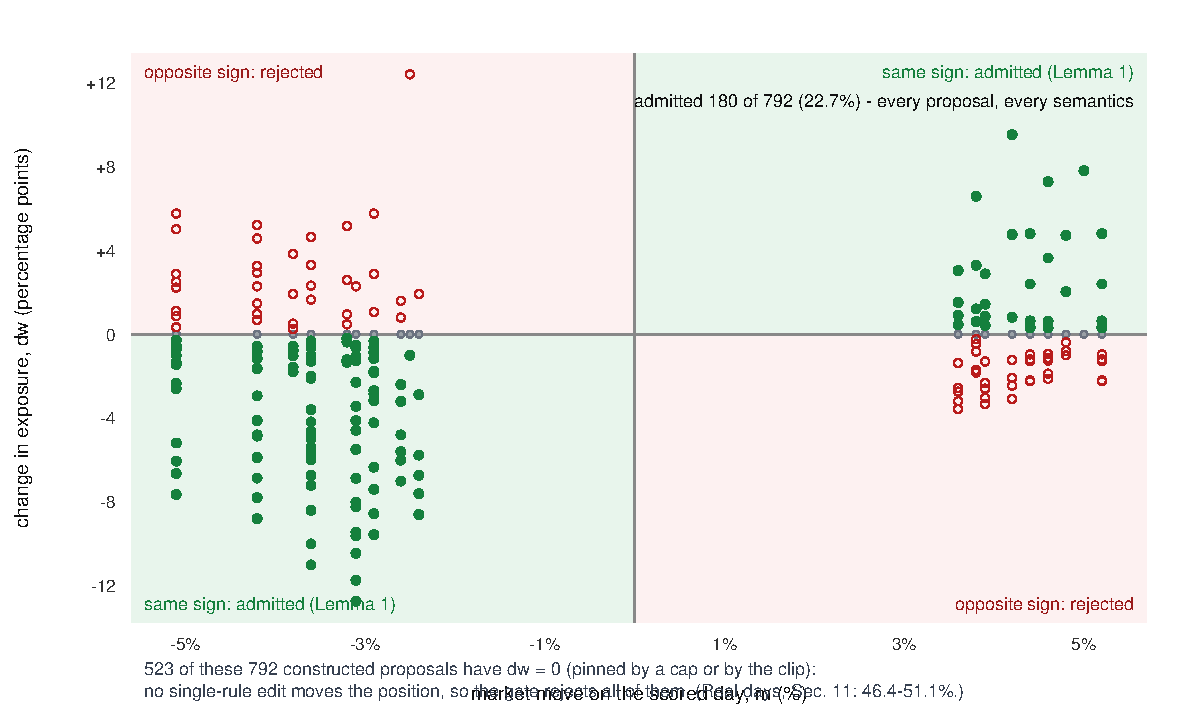
\includegraphics[width=\linewidth]{fig-direction-plane.pdf}
\caption{What a same-day outcome gate can see. Each point is one proposal (one day, one rule, one edit semantics): 792 in total across the four constructed corpora A--D (Sec. 4--5). Horizontally, the market move on the day the re-run is scored; vertically, the change the proposal makes to the position. The gate admits a proposal exactly when the two point the same way (Lemma 1) --- the two shaded quadrants --- and rejects it when they point opposite ways. 523 of the 792 proposals never leave the horizontal axis: the position is pinned by a rule cap or by the 15\% clip, no single-rule edit can move it, and the gate rejects all of them. The gate therefore reads a \emph{direction}, never a reason, and over these constructed corpora two thirds of the proposal space it cannot read at all. Caliber: the no-op share is a property of the corpus that supplies the proposals, not of the gate --- on the four real-day datasets of Sec. 11 the same share is 46.4--51.1\%, and corpus D here is deliberately pinned. \textbf{Two rates appear in this paper and they are not the same fraction:} the 180 of 792 counted here takes \emph{every} proposal of all four corpora under all four semantics, whereas the headline rate quoted in the abstract (48.8\%) counts only \emph{incorrect} edits, over corpora A--C, under one semantics (E2) --- 61 of 125. Same gate, different questions; read them apart. The vertical quantity is written dw in the figure and \(\Delta w\) in the text.}
\label{fig:direction}
\end{figure}

{\def\LTcaptype{none} % do not increment counter
\begin{longtable}[]{@{}
  >{\raggedright\arraybackslash}p{(\linewidth - 8\tabcolsep) * \real{0.2000}}
  >{\raggedright\arraybackslash}p{(\linewidth - 8\tabcolsep) * \real{0.2000}}
  >{\raggedright\arraybackslash}p{(\linewidth - 8\tabcolsep) * \real{0.2000}}
  >{\raggedright\arraybackslash}p{(\linewidth - 8\tabcolsep) * \real{0.2000}}
  >{\raggedright\arraybackslash}p{(\linewidth - 8\tabcolsep) * \real{0.2000}}@{}}
\toprule\noalign{}
\begin{minipage}[b]{\linewidth}\raggedright
\end{minipage} & \begin{minipage}[b]{\linewidth}\raggedright
A (5 \ensuremath{\times} 6)
\end{minipage} & \begin{minipage}[b]{\linewidth}\raggedright
B (8 \ensuremath{\times} 8)
\end{minipage} & \begin{minipage}[b]{\linewidth}\raggedright
C (10 \ensuremath{\times} 8)
\end{minipage} & \begin{minipage}[b]{\linewidth}\raggedright
pooled
\end{minipage} \\
\midrule\noalign{}
\endhead
\bottomrule\noalign{}
\endlastfoot
cells per semantics & 30 & 64 & 80 & 174 \\
\textbf{correct edits passed} & \textbf{4 / 4} & \textbf{6 / 6} & \textbf{9 / 9} & \textbf{19 / 19} \\
\textbf{incorrect edits passed} & \textbf{14 / 20} & \textbf{19 / 42} & \textbf{28 / 63} & \textbf{61 / 125 = 48.8\%} \\
--- on losing days & 13 / 15 & 15 / 21 & 22 / 28 & \textbf{50 / 64 = 78.1\%} \\
--- on ``small-win'' days & 1 / 5 & 4 / 21 & 6 / 35 & \textbf{11 / 61 = 18.0\%} \\
days with no faulty rule --- edits admitted (admitted / candidates) & 6 / 6 & 12 / 16 & 6 / 8 & 24 / 30 \\
\end{longtable}
}

\textbf{Table 1.} Cells per semantics and their verdicts for corpora A--C, pooled in the last column; day-type splits are given for incorrect edits only, and the last row reports the days with no faulty rule.

On a day with no faulty rule \emph{every} rule is a wrong answer, so the last row is the admission rate among wrong answers on those days --- the same quantity as the ``incorrect edits'' row, restricted to no-fault days.

Two properties hold in all three corpora:

\begin{enumerate}
\def\labelenumi{\arabic{enumi}.}
\tightlist
\item
  \textbf{Under the flip semantics, no edit that the key names is rejected} (19/19 pooled). This half is a property of the \textbf{key}, not of the gate: perturbing the key leaves the direction test untouched but degrades this one to 33--100\%, because the generators assert only that \emph{their own} key rule improves the day (§8.5). The invariant that survives every key we tried is the lemma-level one --- \emph{an edit that does improve the day is admitted}.
\item
  \textbf{The pass rate tracks the day type, not the rule at fault}: 71--87\% on losing days versus 17--20\% on small-win days, in each corpus separately --- and this contrast holds under every alternative key we tried, including 1,200 seeded random perturbations (§8.5). §11 shows what that axis \emph{is}: composition read through the day's sign, not a second property of the gate.
\end{enumerate}

One property does not hold: the overall rate. It moves with the corpus, and its value depends on one convention --- whether days with no faulty rule stay in the denominator:

{\def\LTcaptype{none} % do not increment counter
\begin{longtable}[]{@{}
  >{\raggedright\arraybackslash}p{(\linewidth - 6\tabcolsep) * \real{0.2500}}
  >{\raggedright\arraybackslash}p{(\linewidth - 6\tabcolsep) * \real{0.2500}}
  >{\raggedright\arraybackslash}p{(\linewidth - 6\tabcolsep) * \real{0.2500}}
  >{\raggedright\arraybackslash}p{(\linewidth - 6\tabcolsep) * \real{0.2500}}@{}}
\toprule\noalign{}
\begin{minipage}[b]{\linewidth}\raggedright
convention
\end{minipage} & \begin{minipage}[b]{\linewidth}\raggedright
A
\end{minipage} & \begin{minipage}[b]{\linewidth}\raggedright
B
\end{minipage} & \begin{minipage}[b]{\linewidth}\raggedright
C
\end{minipage} \\
\midrule\noalign{}
\endhead
\bottomrule\noalign{}
\endlastfoot
\textbf{incorrect edits only} (days without a faulty rule excluded) & 14/20 = 70.0\% & 19/42 = 45.2\% & 28/63 = \textbf{44.4\%} \\
\textbf{merged} (a day with no faulty rule counts every rule as wrong) & 20/26 = \textbf{76.9\%} & 31/58 = \textbf{53.4\%} & 34/71 = 47.9\% \\
\end{longtable}
}

\textbf{Table 2.} The overall incorrect-edit rate under two denominator conventions --- days without a faulty rule excluded, or merged --- for each corpus.

The first corpus's merged figure (76.9\%) falls \textbf{inside} the band we had pre-registered (60--90\%); the second and third fall below it (53.4\% and 47.9\%). We report both conventions throughout rather than a single rate, and we treat each figure as a property of that corpus's arithmetic and rule mix.

Two further conventions, stated once for the whole paper: \textbf{``correct edit''} means the edit names the key rule on a day that has one; \textbf{``rule''} in §6 means the rule identity (each rule is judged once by the cross-day gate, not once per day).

\section{5. The edit-semantics axis: two regimes, two failure modes}\label{the-edit-semantics-axis-two-regimes-two-failure-modes}

A ``repair'' is not a thing until an implementation says what it does. We sweep four mechanical semantics, all defined on the same day state:

A rule that acted multiplies the day's expected return by its own factor \(f\) (R1 0.3, R2 0.7, R3 0.4, R4 1.2); the two cap-type rules (R5, R6) bound the position directly instead. In what follows \emph{cap} names such a rule-level ceiling, \emph{clip} names the book's 15\% ceiling on a single position, and where it matters we say which one binds. The 15\% ceiling is a parameter of the book (a single-position limit on the portfolio), not an estimate fitted to these data.

{\def\LTcaptype{none} % do not increment counter
\begin{longtable}[]{@{}
  >{\raggedright\arraybackslash}p{(\linewidth - 4\tabcolsep) * \real{0.3333}}
  >{\raggedright\arraybackslash}p{(\linewidth - 4\tabcolsep) * \real{0.3333}}
  >{\raggedright\arraybackslash}p{(\linewidth - 4\tabcolsep) * \real{0.3333}}@{}}
\toprule\noalign{}
\begin{minipage}[b]{\linewidth}\raggedright
semantics
\end{minipage} & \begin{minipage}[b]{\linewidth}\raggedright
on a rule that acted with factor \(f\)
\end{minipage} & \begin{minipage}[b]{\linewidth}\raggedright
on a rule that did not act
\end{minipage} \\
\midrule\noalign{}
\endhead
\bottomrule\noalign{}
\endlastfoot
\textbf{remove} & undo the action (divide \(f\) out) & nothing changes \\
\textbf{flip} & undo the action & make it act (with the rule's own factor, including cap-type rules) \\
\textbf{halve} & apply \(f' = 1+\frac{f-1}{2}\) & nothing changes \\
\textbf{no-leverage} & if \(f>1\), remove the increase; else nothing & nothing changes \\
\end{longtable}
}

\textbf{Table 3.} The four mechanical edit semantics, defined by what they do to a rule that acted and to one that did not act.

Pooled over the three corpora (174 cells each):

{\def\LTcaptype{none} % do not increment counter
\begin{longtable}[]{@{}
  >{\raggedright\arraybackslash}p{(\linewidth - 8\tabcolsep) * \real{0.2000}}
  >{\raggedright\arraybackslash}p{(\linewidth - 8\tabcolsep) * \real{0.2000}}
  >{\raggedright\arraybackslash}p{(\linewidth - 8\tabcolsep) * \real{0.2000}}
  >{\raggedright\arraybackslash}p{(\linewidth - 8\tabcolsep) * \real{0.2000}}
  >{\raggedright\arraybackslash}p{(\linewidth - 8\tabcolsep) * \real{0.2000}}@{}}
\toprule\noalign{}
\begin{minipage}[b]{\linewidth}\raggedright
semantics
\end{minipage} & \begin{minipage}[b]{\linewidth}\raggedright
correct edits passed
\end{minipage} & \begin{minipage}[b]{\linewidth}\raggedright
incorrect edits passed
\end{minipage} & \begin{minipage}[b]{\linewidth}\raggedright
losing days
\end{minipage} & \begin{minipage}[b]{\linewidth}\raggedright
small-win days
\end{minipage} \\
\midrule\noalign{}
\endhead
\bottomrule\noalign{}
\endlastfoot
\textbf{flip} & \textbf{19 / 19 = 100\%} & \textbf{61 / 125 = 48.8\%} & 50 / 64 = 78.1\% & 11 / 61 = 18.0\% \\
remove & 18 / 19 = 94.7\% & 2 / 125 = 1.6\% & 2 / 64 = 3.1\% & 0 / 61 = 0.0\% \\
halve & 15 / 19 = 78.9\% & 2 / 125 = 1.6\% & 2 / 64 = 3.1\% & 0 / 61 = 0.0\% \\
no-leverage & 9 / 19 = 47.4\% & 2 / 125 = 1.6\% & 2 / 64 = 3.1\% & 0 / 61 = 0.0\% \\
\end{longtable}
}

\textbf{Table 4.} Pooled per-semantics verdicts over the three corpora (174 cells per semantics).

The axis is \textbf{not a curve but two regimes}, and the reason is expressiveness rather than magnitude: \texttt{flip} is the only one of the four that \emph{creates} action where none existed, so its proposals actually move exposure. The other three act only where the rule already acted, so most of their proposals are no-ops --- and the gate rejects a no-op by its own definition (``nothing changed today'').

That inverts the failure mode, and the inversion is the finding:

\begin{itemize}
\tightlist
\item
  \textbf{Expressive semantics} (flip): the gate fails by \textbf{admitting wrong attributions} --- 78\% of them on losing days.
\item
  \textbf{Inert semantics} (remove, halve, no-leverage): the gate fails by \textbf{rejecting correct ones} --- up to 53\% of them under no-leverage --- while admitting almost nothing (1.6\%) {[}6{]}.
\end{itemize}

Both failures have the same cause: the gate's verdict is a function of \emph{whether and how exposure moved}, and never of attribution.

\textbf{A pre-registered prediction that failed.} We had written down (before running) that ``no correct edit is rejected'' would hold under all four semantics. It does not: no-leverage keeps only 9 of 19. Per our own rule, the claim is narrowed rather than the criterion moved: \emph{no correct edit is rejected \textbf{by semantics that can express the repair}}; for inert semantics the correct framing is the opposite failure.

\subsection{5.5 When the position is pinned, the gate admits nothing}\label{when-the-position-is-pinned-the-gate-admits-nothing}

The day-type rule in §4 has a precondition that the first three corpora \emph{exercised without our noticing}: \textbf{the edit must be able to move the position}. Counting the proposals by composition alone --- the rule of Result 3, applied as a classifier over the corpora's own specifications --- predicts the admitted count exactly on \textbf{19 of 25 days} across corpora B--E, and every one of the \textbf{six} days it misses is a day whose position is pinned (its pre-cap value sits above a cap or above the 15\% clip: 4.03 \ensuremath{\to} 2.0 in B; 6.72 \ensuremath{\to} 2.0 and 8.80 \ensuremath{\to} 1.0 in C; 14.40 \ensuremath{\to} 2.0 in D; 20.06 \ensuremath{\to} 15.0 and 10.08 \ensuremath{\to} 2.0 in E). So the regime was present in two of the earlier corpora all along, as unanalysed cells; we built a fourth corpus to isolate it and to predict it.

The predictions were written down \textbf{before the corpus existed} (the pre-registration, §9.1): all 24 cell verdicts, with the pinned day predicted at \textbf{1 of 6}.

All 24 cells matched, and the pinned day is the one that matters. Four of its six edits have \(\Delta w\) \textbf{exactly zero} --- removing the discount, removing the leverage, or making another rule act all leave the pre-cap position above the cap, so the gate rejects them as ``nothing changed today'' --- and the one edit that does move the position (removing the cap) \emph{grows} exposure on a losing day, so it is rejected too.

{\def\LTcaptype{none} % do not increment counter
\begin{longtable}[]{@{}
  >{\raggedright\arraybackslash}p{(\linewidth - 6\tabcolsep) * \real{0.2500}}
  >{\raggedright\arraybackslash}p{(\linewidth - 6\tabcolsep) * \real{0.2500}}
  >{\raggedright\arraybackslash}p{(\linewidth - 6\tabcolsep) * \real{0.2500}}
  >{\raggedright\arraybackslash}p{(\linewidth - 6\tabcolsep) * \real{0.2500}}@{}}
\toprule\noalign{}
\begin{minipage}[b]{\linewidth}\raggedright
day
\end{minipage} & \begin{minipage}[b]{\linewidth}\raggedright
type
\end{minipage} & \begin{minipage}[b]{\linewidth}\raggedright
edits admitted
\end{minipage} & \begin{minipage}[b]{\linewidth}\raggedright
four of the six are
\end{minipage} \\
\midrule\noalign{}
\endhead
\bottomrule\noalign{}
\endlastfoot
1 & losing, no cap binding & 3 / 5 incorrect (correct 1/1) & --- \\
\textbf{2} & \textbf{losing, position pinned at the cap} & \textbf{1 / 6} & \(\Delta w = 0\) exactly \\
3 & small-win & 1 / 5 incorrect (correct 1/1) & --- \\
4 & losing, no fault & 5 / 6 & --- \\
\end{longtable}
}

\textbf{Table 5.} Corpus D day by day: edits admitted per day, with the pinned day (six candidates, one admitted) marked.

Two things follow. First, the precondition: \textbf{where the book sits at a cap or at the clip, the gate's failure mode flips from ``admits the wrong edit'' to ``admits nothing''} --- and it does so on a \emph{losing} day, where the ordinary account would predict a high pass rate. Second, the pinned day's verdict is \textbf{independent of the day's sign}, because the edits cannot move the position in either direction. Both follow from Lemma 1; the corpus shows that the arithmetic is not a technicality but a regime the deployed gate will meet whenever a cap or a clip is binding.

A fifth corpus pushes the regime to its other side. \textbf{Corpus E} targets the two variants the earlier corpora did \emph{not} contain: one day whose position is pinned by the \textbf{15\% clip} rather than by a rule's cap (removing either of its two leverages still leaves the pre-cap value above the clip --- 20.06 \ensuremath{\to} 16.72 and \ensuremath{\to} 18.24, both clipped to 15), and one \textbf{up} day whose admitted class is swallowed by a cap. Predictions for all three days --- \textbf{6 / 1 / 6} admitted --- were written before the corpus was generated, and the measurement agrees exactly: on the clip day the gate admits \textbf{6 of 8}, with the two swallowed edits being precisely the two leverages; on the up day it admits \textbf{1 of 8}, and that one is the truth rule (the cap itself). Corpus E is deliberately pinned or control, so it is not part of the pooled census of §4--§5; its own census is \textbf{correct 2/2 · incorrect 5/14 = 35.7\% · no-fault day 6/8}.

\section{6. The cross-day gate: tightening is not discrimination}\label{the-cross-day-gate-tightening-is-not-discrimination}

The second gate specification applies the same edit to every day the rule can reach and accepts only if the total improves \textbf{and no day worsens}. We vary the tolerance (how many days may worsen) and count \textbf{rules} --- one denominator for survivors and for intercepted rules alike:

{\def\LTcaptype{none} % do not increment counter
\begin{longtable}[]{@{}
  >{\raggedright\arraybackslash}p{(\linewidth - 8\tabcolsep) * \real{0.2000}}
  >{\raggedright\arraybackslash}p{(\linewidth - 8\tabcolsep) * \real{0.2000}}
  >{\raggedright\arraybackslash}p{(\linewidth - 8\tabcolsep) * \real{0.2000}}
  >{\raggedright\arraybackslash}p{(\linewidth - 8\tabcolsep) * \real{0.2000}}
  >{\raggedright\arraybackslash}p{(\linewidth - 8\tabcolsep) * \real{0.2000}}@{}}
\toprule\noalign{}
\begin{minipage}[b]{\linewidth}\raggedright
corpus (truth rules / non-truth rules)
\end{minipage} & \begin{minipage}[b]{\linewidth}\raggedright
gate
\end{minipage} & \begin{minipage}[b]{\linewidth}\raggedright
rules accepted
\end{minipage} & \begin{minipage}[b]{\linewidth}\raggedright
truth rules surviving
\end{minipage} & \begin{minipage}[b]{\linewidth}\raggedright
non-truth rules intercepted
\end{minipage} \\
\midrule\noalign{}
\endhead
\bottomrule\noalign{}
\endlastfoot
\textbf{A} (R4 R2 R1 / R3 R5 R6) & \ensuremath{\le}0 worsening days & R1 & \textbf{1 / 3} & \textbf{3 / 3} \\
& \ensuremath{\le}1 & R1 R3 R4 R5 R6 & 2 / 3 & 0 / 3 \\
& \ensuremath{\le}2 & all six & 3 / 3 & 0 / 3 \\
\textbf{B} (R7 R4 R8 R5 R3 / R1 R2 R6) & \ensuremath{\le}0 & --- & \textbf{0 / 5} & \textbf{3 / 3} \\
& \ensuremath{\le}1 & R4 & 1 / 5 & 3 / 3 \\
& \ensuremath{\le}2 & R4 R5 & 2 / 5 & 3 / 3 \\
\textbf{C} (R5 R6 R3 R1 R8 R4 R7 / R2) & \ensuremath{\le}0 & --- & \textbf{0 / 7} & 1 / 1 \\
& \ensuremath{\le}1 & --- & 0 / 7 & 1 / 1 \\
& \ensuremath{\le}2 & R1 R3 R4 & 3 / 7 & 1 / 1 \\
\end{longtable}
}

\textbf{Table 6.} The cross-day gate at three tolerances over corpora A--C, counted in rules: rules accepted, truth rules surviving, non-truth rules intercepted.

Readings:

\begin{enumerate}
\def\labelenumi{\arabic{enumi}.}
\tightlist
\item
  \textbf{Zero tolerance is close to useless as a discriminator}: in B and C it accepts \textbf{no correct rule at all} (0/5, 0/7) while its interception rate stays what it was. The earlier claim (on two corpora) that ``the stricter gate buys interception at the price of correct edits'' is too generous --- in two of three corpora there is nothing to buy: correctness is gone.
\item
  \textbf{The trade-off shape is corpus-dependent}, so it is not a single curve: in A one day of tolerance costs \emph{all} interception (3/3 \ensuremath{\to} 0/3) while recovering only one correct rule; in B interception survives loosening; in C both settings stay empty until tolerance 2.
\item
  Interception cannot be read as a proportion in C at all: seven of eight rules are the key on some day, so only one rule remains in the non-truth class (1/1).
\end{enumerate}

\section{7. What the reader answers contribute, and what we do not claim}\label{what-the-reader-answers-contribute-and-what-we-do-not-claim}

The corpora contain 105 machine-auditable reader answers; only 5 are misattributions of the planted-bait type, and the same-day gate passes 4 of them. With \(n = 5\) these answers cannot estimate a rate, and \textbf{we do not use them to}. Their role is \textbf{existence evidence}: that edits of the kind enumerated in §4 are edits a reader will actually propose. They say nothing about how often such edits arise in a real pipeline, nor about who proposes them.

\textbf{No frequency claim.} We make no claim of the form ``an outcome gate fails on \(x\)\% of real-world proposals'', but a claim about what a gate does with the proposals it is given: on every input it can see, its verdict is a function of the direction of exposure and never of attribution. A frequency claim would need a different corpus --- proposals drawn from a deployed pipeline --- and we say so here rather than leaning on five answers to imply it.

\textbf{What else we do not claim.} We do not claim that any strategy is profitable; that we replicate any prior result; that the reader conditions we compared differ significantly; that tightening a prompt improves attribution; or that we have evaluated SHARP or any deployed gate --- the comparison in §1 concerns what their \emph{reports} claim, not their artefacts. Nor do we claim that tightening a criterion improves discrimination: in our own measurements it removed a class of misattributions (2/6 \ensuremath{\to} 0/5) while reducing correct attributions on another day from 5/5 to 1/5 (\(n = 5\) per side; we pre-registered ``\ensuremath{\ge} 4/5'' and it failed), which we report as a caution rather than a finding. Finally, we do not claim that no deployed pipeline logs per-day proposals with a verdict: a search of public repositories (names, descriptions, and authenticated file-content search) turned up no log of that shape, and the artefacts of the pipeline examined in §11 record \emph{executed} trades plus offline attribution deltas --- missed signals, noise trades, early and late exits, overtrading --- not per-day proposals with a gate decision. That is why §11's external check uses proposals we supply rather than proposals we import, and we say so on every number it reports.

\section{8. Limitations and boundaries}\label{limitations-and-boundaries}

\textbf{8.1} \textbf{Four corpora, four rates, no single rate.} All four are authored; their arithmetic is published and re-checkable, but none is a sample of real markets. Under the two conventions of §4 the incorrect-edit rate is 76.9\% / 53.4\% / 47.9\% (A/B/C, days without a faulty rule merged in) or 70.0\% / 45.2\% / 44.4\% (incorrect cells only), and corpus D --- the smallest --- gives 40.0\%. We report no single rate; that spread, with its convention stated, is the honest width of what we know.

\textbf{8.2} \textbf{Gates are abstractions.} We audit mechanical specifications; a deployed gate may add cooldowns, per-rule budgets or human review. Our claim concerns what outcome information \emph{alone} can contribute.

\textbf{8.3} \textbf{The semantics sweep covers action-type edits only.} All four semantics modify \emph{what a rule did}; none edits conditions, thresholds or the rule set itself. The \textbf{rate findings} of §4--§5 are scoped accordingly, and so are the counting results of §5.5. Lemma 1 itself is not restricted that way: it holds for any edit that changes the position --- including a condition or threshold edit that changes which rules fire --- because the gate's verdict depends only on \((w'-w)m\).

\textbf{8.4} \textbf{Lemma 1 is a restatement} of the same-day gate's definition --- held deliberately as a \textbf{lemma} rather than reported as a discovery. The results are its three consequences (§3) and the corpus tests of them (§5, §5.5).

\textbf{8.5} \textbf{Ground truth is authored --- and we have a number for how far it travels.} Two annotators (same model family; clean one-shot sessions; asked only ``is any rule wrong on this day's facts?'') agree with each other at \ensuremath{\kappa} = 0.714 (Cohen's kappa: chance-corrected agreement, 0 = chance, 1 = perfect; Po = 0.773 over 22 comparable days) but with our key at \textbf{\ensuremath{\kappa} = 0.504} (Po = 0.588 over 17 comparable days). The gap is structured: on corpus C --- built so every criterion is readable --- agreement with the key rises to \textbf{\ensuremath{\kappa} = 0.674} (7 comparable days) and every cell of its ``direct contradiction'' class is found (9/9), while faults requiring judgement of an exhausted trend are found in 1 of 2 comparable cases; the single day whose key is \emph{none} drew, from both annotators, the same rule --- one that never fired. Reproducibility depends on the \emph{shape} of the fault. An artifact audit found 5 of 13 day-cells in the first two corpora whose criterion the material cannot support; we report that separately. We do \textbf{not} claim to have solved the ground-truth problem: the authored key remains part of the estimate's reach, and these numbers are its honest size. What we can do instead is measure \textbf{which of our claims the key can move}. Re-running the census of §4 under alternative keys --- each annotator's answers, each day's planted bait, and 1,200 seeded day-level random perturbations at 20/40/60\% --- leaves the day-type contrast untouched (\textbf{6 of 6 measurable alternative keys, 1,200 of 1,200 random draws}, losing days 75.5--77.6\% versus small-win days 19.6--23.2\%) and leaves the incorrect-edit rate near its baseline (noise medians 46.7 / 48.6 / 50.0\%, 5--95\% band ±3pp). The claim it \emph{does} move is the ``no correct edit is rejected'' half: 100\% under our key in both corpora, but 33.3\% and 20.0\% under two of the alternative keys --- because there ``correct'' means ``the key's rule'', and the generators assert only that their own key rule improves the day (§3). Two further probes answer the natural follow-up. Under an \textbf{annotator-consensus key} (keeping only days where both annotators answered \emph{and agreed}), the result is unchanged where it can be measured --- corpus C: correct edits 7/7, incorrect 22/49 = 44.9\%, losing days 11/14 = 78.6\% versus small-win 6/28 = 21.4\% --- while corpus B is left with a single comparable correct cell, so a harder key buys certainty at the price of \(n\). And stratifying the census by whether the annotators \textbf{disagreed} with our key makes the day-type contrast \emph{stronger} on the contested days (corpus B: 15/21 = 71.4\% versus 2/14 = 14.3\% across the five days where at least one annotator dissented) --- the opposite of what a key artefact would look like.

\textbf{8.6} \textbf{The claim is semantics-scoped} (§5): our pre-registered cross-semantics prediction was falsified and the claim narrowed accordingly.

\textbf{8.7} \textbf{No frequency claim} (§7): what we enumerate are the proposals a gate can be given, not their distribution in any deployed pipeline. The five reader misattributions are used as existence evidence only.

\section{9. Reproducibility}\label{reproducibility}

Every figure above is printed by the accompanying artifact set: corpus generators that self-report their criteria and refuse to write anything if a criterion fails; a scorer with known-answer self-checks and a frozen key whose hash it prints; a reachability audit that decides which day-cells a reader could in principle decide; a key--annotator agreement device with three known-answer self-checks; and the \textbf{semantics sweep}, which reads the corpora' own models from the generators (so no figure is recomputed from a re-typed model) and refuses to print a census unless (i) the recorded positions are reproduced, (ii) its closed-form self-check reports zero inconsistencies across all 792 cells, and (iii) each generator's model dump has exactly days \ensuremath{\times} rules \ensuremath{\times} 4 cells. The fourth corpus is generated by the same family of device and, like the others, refuses to write if its known answers or its ``fix the intended rule improves the day'' assertion fails. The counting rule of Result 3 is tested by a second, independent device (§9.1), which classifies proposals from each generator's own specification fields (which rule fired, discount or leverage or cap, day sign) and prints predicted against measured counts \textbf{per day}, including the days where the two disagree. A third device (§9.1) re-runs the census of §4 under alternative keys and under seeded random key noise, with known-answer self-checks and a bucket-identity assertion (each key's correct + incorrect + no-fault cells must sum to the cells it covers). The artifact set also includes a \textbf{device error log}: which guard caught which mistake, in the order they were caught, together with the regeneration evidence that the export modes cannot mutate a corpus. Both real-day devices of §11 take a \texttt{-\/-csv} argument; running them unchanged on the other three series produces the replication tabulated in the artifact set, and the SPY control reproduces its recorded figures exactly after that parameterization.

No figure here is quoted from memory or from a secondary source.

\subsection{9.1 Data availability}\label{data-availability}

The artifact set is released with this paper and versioned together with the corpora: the five corpus generators (each self-reports its criteria and refuses to write if a criterion fails), the frozen keys and their printed hashes, the scorer, the reachability audit, the semantics sweep, the composition-count and key-sensitivity devices, the device error log, and the 105 auditable reader answers. The design documents referred to in the text are part of the same release --- notably the pre-registration of corpus D, written before that corpus existed (§5.5), and the pre-registrations of the real-day and third-party checks (§11). Every figure is regenerated by one command per table, under the acceptance criteria §9 lists for each device; where the text names a device or a design file directly (\texttt{sweep.mjs}, \texttt{compose-count.mjs}, \texttt{design-corpus-D-prediction.md}), that name resolves to this release. \emph{Release: the artifact set is released as a versioned archive; a DOI will be linked from this section once deposited.}

\section{10. Discussion: implications for a deployed loop}\label{discussion-implications-for-a-deployed-loop}

Our results bound one component --- the outcome signal --- and they translate into five practical statements {[}3, 4, 5{]}.

\begin{enumerate}
\def\labelenumi{\arabic{enumi}.}
\tightlist
\item
  \textbf{Do not use an outcome-only gate to police attribution.} If the loop closes on ``the backtest improved'', the gate's verdict is a function of the direction of exposure that day (§3). It will accept changes aimed at a cause that is not the cause (48.8\% of the misattributions here), and it will do so at a \emph{higher} rate on losing days (78.1\%) --- that is, precisely when such a loop is most likely to be triggered.
\item
  \textbf{Stricter is not sharper.} Refusing any worsening day removes almost all discrimination along with almost all correctness: 1 of 3 correct rules admitted in corpus A, 0 of 5 and 0 of 7 in B and C (§6). Discrimination has to be bought with a different \emph{input}, not a tighter threshold.
\item
  \textbf{Know which failure regime your edit vocabulary puts you in.} Edits that can express a repair produce over-admission; edits that can only undo or attenuate an existing action produce over-rejection --- up to half the correct edits (§5). A team that only counts ``did we ship a bad change'' will never see the second regime.
\item
  \textbf{Instrument the pinned state.} If the position sits at a cap or at the book's 15\% clip, every single-rule edit is a no-op and the gate rejects the entire proposal set --- including on days where a repair existed (§5.5). One comparison (the position before clipping versus after) tells you whether today's proposals are being judged in that regime.
\item
  \textbf{Deployment variants change when the gate is consulted, not what it can see.} Cooldowns, per-rule budgets and human review are scheduling and escalation; they add no information to the outcome channel. The fix that Result 1 implies is to \emph{give the gate an attribution-specific input} --- cross-day consistency, per-rule hit rates, a signed review of the claimed cause --- and the cheapest useful version of that is the bound check of point 4, not a stricter P\&L threshold.
\end{enumerate}

Why the scope of §8.3 does not weaken these statements: they are claims about the \textbf{information content of the outcome signal}, and a condition or threshold edit moves the position just as an action edit does --- the gate sees the movement either way and never sees the reason. What the action-edit restriction does bound is our \emph{census}: the rates we report are rates over action-type proposals, and a different proposal mix would move them (Result 3). The direction, by contrast, is a property of the signal itself.

\section{11. Real days: an external check (first with our own proposals, then with a third party's)}\label{real-days-an-external-check-first-with-our-own-proposals-then-with-a-third-partys}

Everything above is arithmetic over corpora we built, so the natural objection is external validity {[}1{]}. We therefore ran the same gate over \textbf{real market days}, in four datasets (SPY 2000--2016; S\&P 500 2005--2019; S\&P 500 2009--2019; QQQ 2009--2019 --- sources and hashes in the artifact set), with a six-rule book whose rules are mechanical and pre-registered --- two growth rules (trend, 20-day momentum), a volatility discount, an extension leverage, and two caps (drawdown, distance from the moving average) --- and proposals generated by flipping each rule's action, exactly the E2 semantics of §5. Day type is read from the \textbf{market's} move, which is what the gate sees. Note that these are not four independent samples: three of them are views of the same S\&P 500 exposure over overlapping windows, and only QQQ changes the asset.

Two results. The sharp one first: over all \textbf{74,484} cells the gate's verdict equals the closed form of Lemma 1 \textbf{without a single violation in any dataset}, and a second, independently written implementation of the same gate (deciding by counterfactual P\&L rather than by sign) agrees on every cell. The direction also appears on real days, in every dataset: \textbf{33.0\% / 33.7\% / 36.0\% / 37.8\%} admitted on losing days against \textbf{15.7\% / 16.1\% / 15.9\% / 13.3\%} on small-win days (big-up days: 16.4--16.9\%); across the four datasets the ranges are 33.0--37.8\% against 13.3--16.1\%.

The second result is the more useful half, and it is a decomposition. Those gaps --- 17.3, 17.6, 20.1 and 24.5 points --- are not evidence of a \emph{second} property of the gate. In each dataset the admission rate equals the share of proposals whose direction matches the market's move, to within a tenth of a point in almost every bucket (losing days: 33.0/33.0, 33.7/33.7, 36.0/36.0, 37.8/37.8 admitted against shrinking-proposal share). What moves across datasets is the \textbf{composition}: the shrinking share on down days runs 33.0\% to 37.8\%, and it is that number, not the gate, that sets the observed contrast. The day-type contrast of §4--§5 is therefore a property of \textbf{how a corpus was composed}, not a second property of the gate --- which is why §8.3 scopes the \emph{rate} claims to action-type proposals, and why Result 3 predicts rates from composition. A pre-registered prediction of ours said this contrast would be weak in real data; it is not, in any of the four datasets, and the honest reading is the other way round: the contrast is real \emph{as composition}, and its size is a property of the data.

Two readings come free with real data. \textbf{No-op proposals are 46.4--51.1\% of the space} in all four datasets --- in the first corpora that regime was 1 in 6 or 1 in 8. On real days the book usually sits at a cap or at the 15\% clip, so around half of all mechanical proposals cannot move the position at all and the gate's default answer is \emph{reject}. And the days that reject \emph{every} proposal are concentrated in crises: \textbf{158 days (4.0\%)} in the SPY window that contains 2008--2009, 102 (2.9\%) in the 2005--2019 window, but only 13 (0.5\%) and 19 (0.8\%) in the two windows that start at the end of 2008 --- for instance 2008-10-15, drawdown cap binding, weight 2.00\%, market -9.845\%, where the §5.5 mechanism appears on its own, in real data, without being constructed.

\textbf{What this does not establish.} The proposals are ours; only the days and moves are real, and the four datasets are not independent --- three of them are views of the same S\&P 500 exposure over overlapping windows, with QQQ the only different asset. A deployed pipeline's \emph{proposal mix} is the quantity we cannot import: the search of §9 found no public log of per-day proposals with a verdict, and the pipeline we did examine logs executed trades and offline attribution deltas instead. §10's guidance should therefore be read with that boundary in view: the direction is the gate, the rate is the composition.

\subsection{11.1 A third party's proposals}\label{a-third-partys-proposals}

The obvious next step is to stop writing the proposals ourselves. We took a real strategy from a public backtesting library (\texttt{qstrader}) --- its \texttt{MovingAverageCrossStrategy}, a 100/300 simple-moving-average state machine over adjusted closes --- ported it faithfully to daily bars, and treated each of its signals as the proposal, gated on the following day's actual move (a signal computed at the close cannot be credited with the return of the day it was computed on). Note the \emph{sample} first: at its default parameters this strategy proposes \textbf{6, 10, 8 and 6} trades in the four datasets --- six to ten trades in eight to sixteen years. ``A few dozen real proposals'' therefore requires a wider parameter pair, which we use for the numbers below while reporting both (\textbf{20/100: 47, 39, 27 and 25 proposals}); the porting is ours, so this is a third party's \emph{strategy}, not a third party's \emph{run}.

The gate approves \textbf{57.4\%, 46.2\%, 48.1\% and 56.0\%} of those proposals (a 46.2--57.4\% range; 27/47, 18/39, 13/27, 14/25 --- entries 62.5\% / 55.0\% / 57.1\% / 53.8\%, exits 52.2\% / 36.8\% / 38.5\% / 58.3\%), with \textbf{no violations of the closed form} anywhere. The by-type cells show why the headline is what it is: entries are approved on 100\% of up days and 0\% of down days, exits the mirror image, so the only thing that varies is how many entries and exits the strategy happened to place on each kind of day. As a filter, then, the outcome gate sits \textbf{between 46\% and 57\% --- indistinguishable from a coin flip} on a third party's proposals, and our pre-registered guess that the rate would exceed 50\% held in only two of the four datasets. At this sample size the rate is not distinguishable from chance, and neither is any story about the strategy's timing: over \textbf{50 seeded permutations} of the daily returns (proposals and dates held fixed) the approval rate's 2.5--97.5\% band is \textbf{{[}38.3, 63.8{]}} for the 47-proposal sample, and the real figure (57.4\%) falls \textbf{inside} it --- as does every other dataset's real figure (46.2\%, 48.1\% and 56.0\% against bands {[}30.8, 64.1{]}, {[}33.3, 66.7{]} and {[}32.0, 68.0{]}). The closed form stays exact under every permutation: zero violations, in all fifty seeds of all four datasets. What survives is the shape, not the level: the verdict is the direction test, and the level is a small-sample estimate that a few dozen real proposals cannot pin down.

The implication for a deployed loop is the thesis of this paper in someone else's code: what the gate approves is \emph{the day moving your way}, not the reason for the trade --- and whether it approves most of a pipeline's proposals is a statement about that pipeline's direction-calling, not about the gate's ability to catch a misattribution. Where a strategy's direction and the day disagree, the gate rejects the proposal (20 of 47 in the largest of the four samples), and it does so for a reason that has nothing to do with whether the strategy mis-attributed the move.

\textbf{The boundary in one line.} The \emph{direction} is a property of the gate, and it replicates on real data (four datasets, 74,484 cells, zero violations of the closed form). The \emph{rate} is a property of the proposal mix and of the sample size {[}11, 12{]} --- and no deployed pipeline's mix is available to us, in the literature or in the public repositories we could reach (§9).

\section{References}\label{references}

{[}1{]} Y. Wang, H. Zhu, Z. Hu, Y. Yuan, Z. Chen, S. Senthil, H. Hajishirzi, Y. Tsvetkov, P. Dasigi, T. Xiao. \emph{Rethinking the Evaluation of Harness Evolution for Agents.} arXiv:2607.12227, 2026. https://arxiv.org/abs/2607.12227

{[}2{]} J. Shi, S. Tao, Y. Wu, Z. Wang, J. Zhang, et al.~\emph{S3Gym: Can LLMs Turn Self-Testing and Self-Judging into Self-Improvement?} arXiv:2608.31100, 2026. https://arxiv.org/abs/2608.31100

{[}3{]} X. Chen, W. Zhu, S. Zheng, K. Rasul, Y. Deng, H. Li. \emph{SHARP: A Self-Evolving Human-Auditable Rubric Policy for Financial Trading Agents.} arXiv:2605.06822, 2026.

{[}4{]} S. Kim, Y. Choi, M. Kang, S. J. Hwang. \emph{EvolveTrade: Experience-Driven Policy Refinement for Self-Evolving LLM Trading Agents.} arXiv:2609.17632, 2026.

{[}5{]} J. Mao, C. Li, X. Li, Q. Duan, J. Yuan, et al.~\emph{EVOQUANT: Self-Evolving Verifier-Guided Strategy Optimization for Robust Quantitative Trading.} arXiv:2607.12455, 2026.

{[}6{]} J. Jiang, Y. Xiong. \emph{Can defects be fixed with weak test suites? An analysis of 50 defects from Defects4J.} arXiv:1705.04149, 2017.

{[}7{]} B. J. D. Gort, X.-Y. Liu, X. Sun, J. Gao, S. Chen, C. D. Wang. \emph{Deep Reinforcement Learning for Cryptocurrency Trading: Practical Approach to Address Backtest Overfitting.} arXiv:2209.05559, 2022.

{[}8{]} A. Koshiyama, N. Firoozye. \emph{Avoiding Backtesting Overfitting by Covariance-Penalties: an empirical investigation of the ordinary and total least squares cases.} arXiv:1905.05023, 2019.

{[}9{]} H. White. \emph{A Reality Check for Data Snooping.} Econometrica, 68(5):1097--1126, 2000. DOI 10.1111/1468-0262.00152

{[}10{]} D. H. Bailey, M. López de Prado. \emph{The Deflated Sharpe Ratio: Correcting for Selection Bias, Backtest Overfitting, and Non-Normality.} The Journal of Portfolio Management, 40(5):94--107, 2014. DOI 10.3905/jpm.2014.40.5.094

{[}11{]} C. R. Harvey, Y. Liu, H. Zhu. \emph{\ldots and the Cross-Section of Expected Returns.} The Review of Financial Studies, 29(1):5--68. DOI 10.1093/rfs/hhv059 (Crossref records the issue year as 2015; the printed issue is dated 2016 --- use the venue's own convention in the formal package.)

{[}12{]} A. Y. Chen, T. Zimmermann. \emph{Publication Bias in Asset Pricing Research.} arXiv:2209.13623, 2022.

{[}13{]} W. Wang, P. Piękos, L. Nanbo, F. Laakom, Y. Chen, et al.~\emph{Huxley-Gödel Machine: Human-Level Coding Agent Development by an Approximation of the Optimal Self-Improving Machine.} arXiv:2510.21614, 2025.

\section{Appendix A --- the artifact set}\label{appendix-a-the-artifact-set}

Four corpora with rule sets and frozen keys; the devices named in §9; the frozen transcripts of the annotator sessions behind the \ensuremath{\kappa} figures; and the 105 auditable reader answers. The sweep's cell-level output (792 rows) is reproducible with one command.

\section{Use of AI tools}\label{use-of-ai-tools}

The corpora, the measurement devices, the analyses and the first draft of this paper were produced by an agent (D, a text-to-text generative tool) running inside the author's own deployment, under the author's direction. The agent also ran the annotator sessions reported in §8.5 and computed the agreement statistics. The human author is the sole author of this paper; she directed the work, checked the artifacts, decided what may be claimed, and takes full responsibility for the content.

\end{document}
